\chapter{Literature Review}
 \thispagestyle{myheadings}
Current adult image filtering techniques can be classified into three categories: keyword based, blacklist based and content based. Our proposed system is content based i.e. images will be classified on the basis of their content. The classification approach we applied can be broadly classified into two categories- Skin based and non-skin based.

%
\section{Skin Based Approach}
Our human civilization has been influenced and intoxicated by the web
revolution. People of every age use the web for different needs and purposes. Some use it for fun; some use it for their studies and find information while some live on it. Images are essentially part of the modern web and we all agree to the fact that a single picture is worth thousand words. We can find all sort of information on the web and it has been a part of our daily life. However, it also has abundance of images and contents that may be unsuitable for certain age groups. Finding pornographic images posted on social sites and links on study groups is not a new thing in today's world. Pornographic images certainly need to be managed and unavailable to children and men at work.


 



\subsection{Skin Color Detection Method}
The most important feature that provides clues to image content is color. Color is a low level feature, which makes it computationally inexpensive and therefore suitable for real-time object characterization, detection and localization. Generally pornographic images show a lot of skin and thus skin color is a basic feature used in detecting pornographic images. The main goal of skin color detection or classification is to build a decision rule that will discriminate between skin and non-skin pixels. Identifying skin colored pixels involves finding the range of values for which most skin pixels would fall in a given color space


\subsubsection{Color Spaces}
The purpose of a color space is to facilitate the specification of colors in some standard, generally accepted manner. A color space is a specification of a coordinate system and subspace within a system where each color is represented by a single point. Various color spaces are used for processing digital images. For some purposes, one color space may be more appropriate than others.  

\subsubsection{The RGB Color Space}
The RGB color space originated from CRT display applications.  In the RGB space each color appears in its primary spectral component of red, green, and blue.  Images represented in the RGB space consist of three component images, one for each primary color.  When fed into an RGB monitor, these images combine on the phosphor screen to produce a composite  color image (Gonzalez and Woods, 2002).The RGB color space is one of the most widely used color spaces for storing and processing digital image.  However, the RGB color space alone is not reliable for identifying skin-colored pixels since it represents not only color but also luminance.  Skin luminance may vary within and across persons due to ambient lighting so it is not dependable for segmenting skin and non-skin regions.   Chromatic colors are more reliable and these are obtained by eliminating luminance through some form of transformation.  The color spaces Normalized RGB, HSV, and YCbCr are transformations commonly used by studies on skin color (Waibel et al., 1999).


\subsubsection{The HSV Color Space}
The HSV (Hue, Saturation, Value/Intensity/Luminance) color space describes
color with intuitive values, based on the artist's idea of tint, saturation and tone.  This was introduced when there was a need to specify color properties numerically.  Hue defines the dominant color as described by wavelength, for instance the distinction between red and yellow.   Saturation measures the colorfulness of an area in proportion to its brightness such as the distinction between red and pink.   Value refers to the color luminance, the distinction between a dark red and a light  red. For skin detection, the value component is discarded to eliminate the undesirable effect of uneven illumination.  The transformation is defined by

\begin{align}
H&=\arccos\frac{\frac{1}{2} (R-G)+ (R-B)}{\sqrt{(R-G)^2 + (R-B)(G-B)}}\\
S&=1-\frac{3min(R,G,B)}{R+G+B}\\
V&=\frac{R+G+ B}{3}
\end{align}

Some studies show that HSV is invariant to highlights at white light sources, to matte surfaces, and ambient lighting. However, hue discontinuities and the computation of the luminance component conflict badly with the properties of color vision.

\subsubsection{The YCbCr Color Spacr}
YCbCr is a family of color spaces used as a part of the color image pipeline in video and digital photography systems. Y' is the luma component and CB and CR are the blue-difference and red-difference chroma  components. Y' (with prime) is distinguished from Y which is luminance, meaning that light intensity is non-linearly encoded using gamma.

Y'CbCr is not an absolute color space, it is a way of encoding RGB information.
The actual color displayed depends on the actual RGB colorants used to display the signal. Therefore a value expressed as Y'CbCr is only predictable if standard RGB colorants or an ICC profile are used.The transformation from RGB to YCbCr is defined by
\begin{align}
Y'&=16+ (65.481R + 128.553G + 24.966B)\\
Cb&=128+(-37.797R- 74.203G +112B)\\
Cr&=128+(112R -93.786G - 18.214B)
\end{align}
%

\subsubsection{Procedure}

We have implement skin based classifier for nudity detection in Images. Skin based implementation composed of
\begin{itemize}
\item Skin segmentation algorithm

\item  Feature selection and SVM training
\end{itemize}

\subsubsection{Skin Segmentation Algorithm}
Skin segmentation is widely used in human and face detection applications. Histogram based algorithm are very popular due to its proved efficiency.

Histogram density for skin and non-skin pixels is calculated from the dataset (Compaq Dataset and manually collected images).The color of skin in the visible spectrum depends primarily on the concentration of melanin and hemoglobin. Distribution of the skin colors is affected by the ethnicity an illumination conditions. However, under arbitrary conditions of illumination the variation in skin color will be less constrained. Given a sufficiently large collection of labeled images captured under a wide variety of imaging conditions, we can model the distribution of skin and non-skin colors accurately.

We constructed skin and non-skin histogram models using our classifier training
set of images.  Given skin and non-skin histograms we can compute the probability that a given color value belongs to the skin and non-skin classes:
\begin{align}
P(rbg|skin)=\frac{s[rgb]}{T_{s}} \\
P(rbg|\neg skin)=\frac{n[rgb]}{T_{n}}
\end{align}

where s[rgb] is the pixel count contained in bin rgb of the skin histogram, n[rgb]  is the equivalent count from the non-skin histogram, and ${T_{s}}$ anmd ${T_{n}}$ are the total counts contained in the skin and non-skin histograms, respectively.

From the skin and non-histogram models we can construct skin pixel classifier. Skin pixel classifier can be mathematically expressed in terms of likelihood ratio as:
\begin{align}
            \frac{P(rgb|skin)}{ P(rgb|\neg skin)}\ge\theta
\end{align}
Where $ 0\le\theta\ge1 $ is the threshold and can be adjusted to trade-off between correct detections and false positives. We can write  as $\theta$ a function of the priors and the cost of false positives and false negatives:


\begin{align}
\theta=\frac{c_{p}P(\neg skin)}{ c_{n}P(skin)}
\end{align}
     
Where ${c_{p}}$ and ${c_{n}}$ are the application-dependant cost of false positives and false negatives, respectively. One reasonable choice of priors is $P(skin)= {T_{s}}/({T_{s}}+{T_{n}})$.
Using the likelihood equation each pixel in and image can be classified as skin or non-skin.
\par
We also implemented gaussian mixture model for skin detection. we used
precomputed mixture parameter \cite{Statistical}.It was found that gaussian
mixture model is computationally expensive and doesn't fit into our performance requirement.
 
\subsubsection{Feature selection and SVM training}
            We computed feature vector from the output of the skin detector and trained a classifier on these features to
             determine whether the image is adult or not. We tested for different set of features vector 
             consisting of Percentage of pixels detected as skin, Average probability of the skin pixels, 
             size in pixels of the largest connected component of skin, Number of connected components of skin etc. 
             However, the system didn't meet our desired accuracy.

\subsection{Gaussian Mixture Model}
Mixture model is a probabilistic model for density estimation. A mixture model can be regarded as a 
type of unsupervised learning. Mixture models consist of collection of component function, usually 
Gaussian. These component functions are combined to provide a multimodal density. They can be employed
 to model the skin colour distribution in order to perform colour-based skin segmentation. A mixture
  density function is expressed as the sum of gaussian kernels:
\begin{align}
P(x)=\sum_{i=0}^N w_{i} \frac{1}{(2\pi)^\frac{3}{2} \|\sum_{i}\|^\frac{1}{2}}
e^ \frac{1 (x-\mu_{i})^T \sum_{i}^-1(x-\mu_{i})}{2} ,
\end{align}
Where x is an RGB color vector and the contribution of $i^{th}$  Gaussian is
determined by a scalar weight $w_{i}$ , mean vector $\mu_{i}$ and diagonal
covariance matrix $\sum_{i}$ .

For modeling skin and non skin classes 16 Gaussian models were used. During
this project we used pre-computed \cite{Statistical} Gaussian parameter for skin
and non skin models.

\begin{table}[h]
\begin{tabular}{|c|c|c|c|}
\hline
Kernel &Mean &CoVariance &Weight \\ \hline

1 &(73.53,29.94,17.76) &(765.40,121.44,112.80) &0.0294 \\
2 &(249.71,233.94,217.49) &(39.94,154.44,396.05) &0.0331 \\
3 &(161.68,116.25,96.95) &(291.03,60.48,162.85) &0.0654 \\
4 &(186.07,136.62,114.40) &(274.95,64.60,198.27) &0.0756 \\
5 &(189.26,98.37,51.18) &(633.18,222.40,250.69) &0.0554 \\
6 &(247.00,152.20,90.84) &(65.23,691.53,609.92) &0.0314 \\
7 &(150.10,72.66,37.76) &(408.63,200.77,257.57) &0.0454 \\
8 &(206.85,171.09,156.34) &(530.08,155.08,572.79) &0.0469 \\
9 &(212.78,152.82,120.04) &(160.57,84.52,243.90) &0.0956 \\
10 &(234.87,175.43,138.94) &(163.80,121.57,279.22) &0.0763 \\
11 &(151.19,97.74,74.59) &(425.40,73.56,175.11) &0.1100 \\
12 &(120.52,77.55,59.82) &(330.45,70.34,151.82) &0.0676 \\
13 &(192.20,119.62,82.32) &(152.76,92.14,259.15) &0.0755 \\
14 &(214.29,136.08,87.24) &(204.90,140.17,270.19) &0.0500 \\
15 &(99.57,54.33,38.06) &(448.13,90.18,151.29) &0.0667 \\
16 &(238.88,203.08,176.91) &(178.38,156.27,404.99) &0.0749 \\
\hline
\end{tabular}
\caption{Mixture Of Gaussian Skin Color model}
\label{tab:GMMSkin}
\end{table} 

\newpage

\begin{table}[h]
\begin{tabular}{|c|c|c|c|}
\hline
Kernel &Mean &CoVariance &Weight \\ \hline
1 &(254.37,254.41,253.82) &(2.77,2.81,5.46) &0.0637 \\
2 &(9.39,8.09,8.52) &(46.84,33.59,32.48) &0.0516 \\
3 &(96.57,96.95,91.53) &(280.69,156.79,436.58) &0.0864 \\
4 &(160.44,162.49,159.06) &(355.98,115.89,591.24) &0.0636 \\
5 &(74.98,63.23,46.33) &(414.84,245.95,361.27) &0.0747 \\
6 &(121.83,60.88,18.31) &(2502.24,1383.53,237.18) &0.0365 \\
7 &(202.18,154.88,91.04) &(957.42,1766.94,1582.52) &0.0349 \\
8 &(193.06,201.93,206.55) &(562.88,190.23,447.28) &0.0649 \\
9 &(51.88,57.14,61.55) &(344.11,191.77,433.40) &0.0656 \\
10 &(30.88,26.84,25.32) &(222.07,118.65,182.41) &0.1189 \\
11 &(44.97,85.96,131.95) &(651.32,840.52,963.67) &0.0362 \\
12 &(236.02,236.27,230.70) &(225.03,117.29,331.95) &0.0849 \\
13 &(207.86,191.20,164.12) &(494.04,237.69,533.52) &0.0368 \\
14 &(99.83,148.11,188.17) &(955.88,654.95,916.70) &0.0389 \\
15 &(135.06,131.92,123.10) &(350.35,130.30,388.43) &0.0943 \\
16 &(135.96,103.89,66.88) &(806.44,642.20,350.36) &0.0477 \\
\hline
\end{tabular}
\caption{Mixture Of Gaussian Non-Skin Color model}
\label{tab:GMMNonSkin}
\end{table} 


\section {Non Skin Based Approach}


\subsection {BIC}
BIC is a pixel classification algorithm that labels pixels into two categories Border and Interior. BIC is based upon Point image processing algorithm.

The BIC approach basically composed of three main components:
\begin{itemize}
\item a simple and powerful image analysis algorithm that classifies image pixels as border or  interior

\item a logarithmic distance to compare histograms

\item a compact representation for the visual features extracted from images.

\end{itemize}
 

Image Analysis

 

BIC image analysis algorithm relies on the RGB color-space uniformly quantized in 4X4X4=64 colors. BIC can be implemented using other color-space quantization for eg. YCbCr, HSV etc. After the quantization step, image pixels are classified as border or interior pixels. A pixel is classified as border if it is at the border of the image itself or if at least one of its 4-neighbors (top, bottom, left and right) has a different quantized color. A pixel is classified as interior if its 4-neighbors have the same quantized color. It is important to observe that this classification is mutually exclusive (either a pixel is border or it is interior) and it is based on a inherently binary visual property of the images. We choose 4-neighbors instead of 8-neighbors because, given the simplicity and generality of the problem, the use of 4-neighbors is able to reduce the image analysis complexity without perceptual losses in terms of retrieval effectiveness.

After the image pixels are classified, one color histogram is computed considering only border pixels, and another color histogram is computed considering only interior pixels. In this way, we have the border/interior classification represented for each quantized color.

\begin{figure}[h]
\centering
  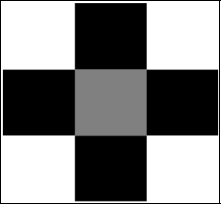
\includegraphics{BIC}
  \caption  {Neighbour BIC Classification}
   \label{BIC}
\end{figure} 

Grayed pixel as shown in figure is classified by comparing to its four neighbors (black squares)
 to classify whether the pixel is interior or Boundary. A pixel is classified as interior if its 
 4-neighbors have the same quantized color. It is important to observe that this classification is 
 mutually exclusive (either a pixel is border or it is interior). The four neighboring BIC 
 classification can be extended to 8- neighbor scheme. However due to the simplicity and performance 
 we choose 4-neighbors scheme 
 

Logarithmic Distance function

Image analysis algorithm describes an image by the means of two color histogram with 64 bins. Two histogram can be combined into a single histogram with 64 bins so that vectorical distance function like L1-Norm and L2-Norm can be used to compare the visual features.

Vectorical distances have also well-known limitations. One of such limitations is that a high value in a single histogram bin dominates the distance between two histograms, no matter the relative importance of this single value.To avoid the problem of high values in a single histogram bin dominate the distance between two histograms, the dLog distance function is used. This function uses a logarithm scale reducing 28 times the range of distances between the smallest and the largest histogram bin values, given that in the log-scale a bin is normalized in the interval [0,9].

The dLog function compares histograms in a logarithmic scale, and is defined as:
\begin{align}
dLog(q,d) = \sum_{i=0}^M |f(q[i])- f(d[i])|\label{dLog}   \\
f(x)= \left\{ 
\begin{array}{l l}
  0 & \quad \mbox{if $x$ =0}\\
  1 & \quad \text {if } 0< x \le 1\\ 
  |\log_{2}{x}| & \quad \text{,otherwise} \\
\end{array} \right.
\end{align}

In the given equation \ref{dLog}, q and d are two histograms with M bins each. The value q[i] represents the $ i^{th}$ bin of histogram q and d[i] represent the $i^{th}$ bin of histogram d. The histogram bins are normalized between 0 and 255.

 

The comparison of histograms with the dLog function does not solve the problem of histogram bins with very high values, but diminishes its effects in most of the situations. In a log-scale, the difference between the largest and the smallest distances between histogram bins becomes smaller than in the original scale. In the original scale, the smallest distance between histogram bins is zero (both images have the same amount of a particular color) and the largest distance is 255 (when the images have just one color and they are different). In our log-scale, the smallest distance is 0 and the largest distance is just 9. The range of distances in the original scale is thus 255=9 = 28 times larger than in the proposed log-scale.

 

 

Compact Visual Features Representation

After applying the DLog function we obtain one histogram with 2XQ bins where each bin contains integer values between 0 and 9.Each image is compactly represented by this histogram vector where each position represents a bin. Thus produced compact representation of the images can be directly plugged into SVM as a features vector.

 

 

\clearpage
\subsection {MPEG-7}



The MPEG-7 standard\cite{Mpeg} is an international standard since September 2001
which specifies metadata for describing multimedia content. The interest-
ing part for our project is this part of the standard which defines visual
descriptors. These are structures to describe multimedia data. Their exact
extraction methods are not standardized.  shows an overview of
MPEG-7 visual descriptors which are suitable for still images.
Since 2001, lots of research has been conducted on making use of these
standardized visual descriptors in the field of Computer Vision, especially in
Content-Based Image Retrieval Systems 
\begin{figure}[h]
  \centering
  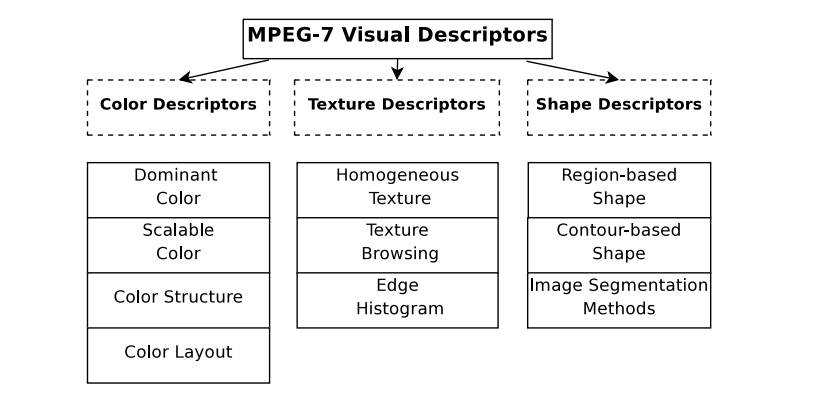
\includegraphics[width=6in]{Mpeg7}
  \caption  {MPEG-7 Visual Descriptors For Low-level Features.}
   \label{Mpeg7}
\end{figure}


\subsubsection {Dominant ColorDescriptor}
Dominant Color Descriptor  (DCD) provides an effective, 
compact  and  intuitive  description  of  the  representative 
colors  in  an  image or  region  . The descriptor  consists 
of  the  Color  Index  (ci),  Percentage  (pi),  Color Variance 
(vi) and Spatial Coherency (s); the last two parameters are 
optional.  Then the DCD is defined by: 
\begin{align}
F={(c_{i},p_{i},v_{i}),s}, i=1,....,N
\end{align} 
where N is the number of the colors and                      . 
For dominant  color  extraction,  the  generalized Lloyd 
algorithm  is  used  for  color  clustering. 
There is one overall Spatial Coherency (SC) value for the 
whole  image  and  several  groups  of $(c_{i},  p_{i},  v_{i}) $  for  the 
corresponding dominant colors. The  Perceptual  colors  to  represent  images  based  on  dominant colors  \ref{DCD}
\begin{table}[h]
\begin{tabular}{| c | c | c |c |}
\hline
S/No.              & Red &Green &Blue   \\
\hline
Manchester United & 6 & 4 & 0   \\
Celtic            & 6 & 3 & 0    \\
FC Porto           & 6 & 2 & 1   \\
FC Copenhagen     & 6 & 2 & 1  \\
\end{tabular}
\caption{ Perceptual  colors  to  represent  images  based  on  dominant colors }
  \label{DCD}

\end{table}
\subsubsection{DCD Extraction}
The  extraction  procedure  for  the dominant  color  uses  the Generalized
Lloyd Algorithm (GLA)\cite{vector}  to  cluster  the  pixel  color  values.
After  defining  the  colors,  for  each  image implement the following steps:
\begin{itemize}
\item Read  in  the  image  and  create  an  image  array  that 
contains  the RGB components of each pixel  in  the 
image
\item For each pixel in the image do: 
	\begin{itemize}
	\item Search  color  table  for  the  nearest  color  by finding  the distance between  the pixel  color  I 
		represented as  $(P_{r}, P_{g}, P_{b})$ and  the color  in  the color  table $ C_{i}$  represented  as 
		$(C_{iR},  C_{iG},  C_{iB})$ using the distance formula (3): 
		\[  C_{d}=(\sqrt{(P_{r}-C_{ir})^2 + (P_{g}-C_{ig})^2 + (P_{b}-C_{ib})^2}), \]
                        \qquad  i=1,2....18
	\item Assign  to  the  pixel  the  RGB  entry  in  color table for which $C_{d}$ is the minimum
	\end{itemize}
\item Create a frequency table for each assigned color 
\item Sort  the  frequency  table  in  descending  order MPEG-7  DCD  allows  at  most  eight  colors  to  be 
	represented.The  highest  four  frequent colors  are  then  selected  with  their  percentages  to 
	create the description of the image.
\end{itemize}


\subsubsection{Edge Histogram Descriptor}
The EHD represents the spatial distribution of edges in an image. The extraction process of the EHD consists of the following stages:
\begin{itemize}
\item The edges in each image-block is categorized into one of the following
	six types: vertical, horizontal, 45 degree diagonal, 135 degree diagonal,
	nondirectional edge and no-edge. (See Figure 8)
\item Now a 5-bin edge histogram of each subimage can be obtained. (See \ref{ehd})
\item Each bin value is normalized by the total number of image-blocks in the image.
\item The normalized bin values are nonlinearly quantized.
\begin{figure}[htp]

     \subfigure [Horizontal Edge]{\label{ehd-a} \includegraphics[scale=0.60]{{horizontal}}}
   \qquad \subfigure[Vertical Edge]{\label{ehd-b}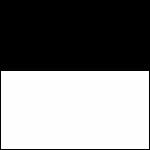
\includegraphics[scale=0.6]{vertical}} 
  \qquad    \subfigure[45 degree edge ]{\label{ehd-c}
\includegraphics[scale=0.6]{diagonal}} \\ 
	\subfigure [135 degree edge] {\label{ehd-d}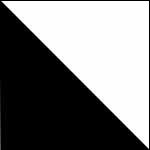
\includegraphics[scale=0.6]{135}}
\qquad \subfigure [non-directional edge] {\label{ehd-e}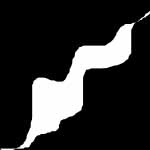
\includegraphics[scale=0.6]{no-direction}}

  \caption{Five types of Edges}
  \label{ehd}
\end{figure}
\end{itemize}

\subsubsection{Color Structure descriptor}
%
This descriptor expresses local color structure in an image
using an 8 x 8-structuring element. It counts the number of
times a particular color is contained within the structuring
element as the structuring element scans the image. Suppose
$c_{0},c_{1},c_{2},\ldots c_{M-1} $ denote the M quantized colors. A color
structure histogram can then be denoted by $h(m)$,m=0,1,2,\ldots M-1 where the
value in each bin represents the number of structuring elements in the image containing one
or more pixels with color $c_{m}$. The HMMD color space is used
in this descriptor.
\begin{table}[h]
\begin{tabular}{| c | c | c |c |}
\hline
S/No.              & Red &Green &Blue   \\
\hline
Manchester United & 6 & 4 & 0   \\
Celtic            & 6 & 3 & 0    \\
FC Porto           & 6 & 2 & 1   \\
FC Copenhagen     & 6 & 2 & 1  \\
\end{tabular}

\caption{ HMMD COLOR SPACE QUANTIZATION FOR CSD }
\label{HMMD-table}
\end{table}
The CSD is defined using four color space quantization oper-
ating points: 184, 120, 64, and 32 bins. To construct a 184-level
quantized color, HMMD color space is quantized nonuniformly
as follows. The whole HMMD color space is divided into five
subspaces. This sub-space division is performed on the diff pa-
rameter (see Section III-A). For the respective subspaces, uni-
form color quantization on the Hue and Sum values results in a
184-level color quantization. The number of quantization levels
for each subspace for different number of histogram bins is
given in table ~\ref{HMMD-table}. \\

In order to compute the CSD, an 8x8-structuring element is used. Even though the
total number of samples is kept fixed at 64, the spatial extent of the structuring element scales with
the image size. The following simple rule determines the spatial
extent of the structuring element (equivalently, the sub sampling
factor) given the image size:
\begin{align}
	&p=max \{0,round(0.5log_{2}WH-8)\} \nonumber \\
	&k=2^p, E=8K                     
\end{align}
where\\
W,H \quad image width and height, respectively;\\
ExE \quad spatial extent of the structuring element; \\
K   \qquad sub-sampling factor.\\
For images smaller than 256x256 pixels, an 8x8 element
with no sub-sampling is used. As another example, if the image
size is 640x480, then p=1,K=2 and E=16. So,
every alternate sample along the rows and columns of a 16x16
-structuring element is then used to compute the histogram.
\\
Each bin of the CSD h(m) represents
the number of locations of the structuring element at which a
pixel with color $c_{m}$ falls inside the element. The origin of the
structure element is defined by its top-left sample. The locations
of the structure element over which the descriptor is accumu-
lated are defined by the grid of pixels of the possibly sub-sam-
pled input image.Structurin element is as shown in fig~\ref{fig:structuring_element} 

\begin{figure}[h]
\centering
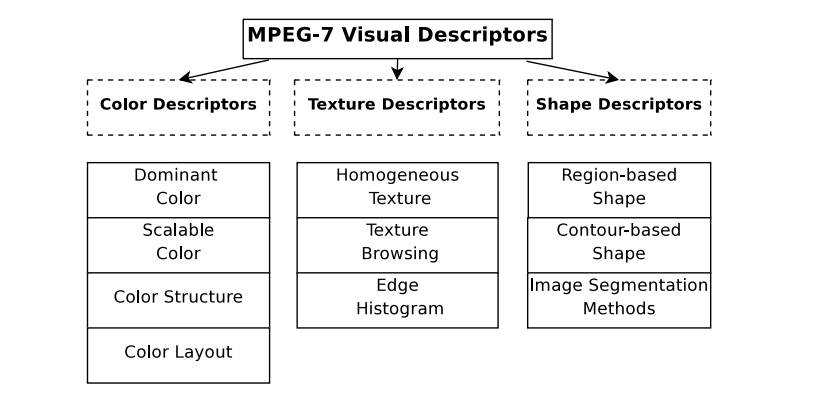
\includegraphics[width=5in]{Mpeg7}
\caption{Structuring element for images}
\label{fig:structuring_element}
\end{figure}
%






\subsubsection{Scalable Color Descriptor}
%
The SCD addresses the interoperability issue by fixing the color space to HSV, with a uniform quantization of the HSV space to 256 bins.
The bin values are nonuniformly quantized to a 11-bit value. \\
This method achieves full interoperability between different
resolutions of the color representation, ranging from 16 bits/histogram at the low end to approximately 1000 bits/histogram at
the high end.Of course, the accuracy of the feature description is
highly dependent on the number of bits used. However, core experiments have shown that good retrieval results are still achievable using only 64 bits, while excellent results can be obtained
using medium or full resolution of the descriptor. \\
The HSV space is uniformly quantized into a total of 256
bins. This includes 16 levels in H, four levels in S, and four
levels in V. The histogram values are truncated into a 11-bit
integer representation. To achieve a more efficient encoding, the
11-bit integer values are first mapped into a ``nonlinear" 4-bit representation, giving higher significance to the small values
with higher probability.
This 4-bit representation of the 256-bin HSV histogram
would require 1024 bits/histogram, which is too large a number
in the context of many MPEG-7 applications. To lower this
number and make the application scalable, the histograms are
encoded using a Haar transform.
The basic unit of the Haar transform consists of a sum oper-
ation and a difference operation [see Fig. 4(a)], which relate to
primitive low- and high-pass filters. Summing pairs of adjacent
histogram lines is equivalent to the calculation of a histogram
with half number of bins.\\
The high-pass (difference) coefficients of the Haar transform
express the information contained in finer-resolution levels
(with higher number of bins) of the histogram. Natural image
signals usually exhibit high redundancy between adjacent
histogram lines. This can be explained by the “impurity”
(slight variation) of colors caused by variable illumination and
shadowing effects. Hence, it can be expected that the high-pass
coefficients expressing differences between adjacent histogram
bins usually have only small values. Exploiting this property,
it is possible to truncate the high-pass coefficients to integer
representation with only a low number of bits.\\
The high-pass (difference) coefficients of the Haar transform
express the information contained in finer-resolution levels
(with higher number of bins) of the histogram. Natural image
signals usually exhibit high redundancy between adjacent
histogram lines. This can be explained by the ``impurity''
(slight variation) of colors caused by variable illumination and
shadowing effects. Hence, it can be expected that the high-pass
coefficients expressing differences between adjacent histogram
bins usually have only small values. Exploiting this property,
it is possible to truncate the high-pass coefficients to integer
representation with only a low number of bits.
\begin{table}
\centering
\begin{tabular}{|c|c|}
	
a &b \\
c &d  \\
e &f  \\
\end{tabular}
\label{tab:CSD}
\caption{EQUIVALENT PARTITIONING OF THE HSV COLOR SPACE}
\end{table}
%
\subsubsection {Edge and Moment Appraoch}

\subsubsection{Edge Detection}
An edge in an image is a contour across which the brightness of the image changes abruptly.
In image processing, an edge is often interpreted as one class of singularities. In a function,
singularities can be characterized easily as discontinuities where the gradient approaches
infinity. However, image data is discrete, so edges in an image often are defined as the
local maxima of the gradient.
\\
Edge detection is an important task in image processing. It is a main tool in pattern
recognition, image segmentation, and scene analysis. An edge detector is basically a high-
pass filter that can be applied to extract the edge points in an image.

\subsubsection{Classical Edge Detectors}
Many classical edge detectors have been developed over time. They are based on the
principle of matching local image segments withspecificedgepatterns. Theedgedetection
is realized by the convolution with a set of directional derivative masks.The popular edge detection operators are Roberts, Sobel, Prewitt, Frei-Chen, and Laplacian operators
Creating a footnote is easy.\footnote{An example footnote.}  	an example footnote.
\subsubsection{Sobel Edge Detector}

\[
G_{x}=
 \begin{bmatrix}
  +1 &+2 &+1 \\
  0 & 0 & 0 \\
  -1 & -2 & -1
 \end{bmatrix} *A
\]
\[
G_{y}=
 \begin{bmatrix}
  +1 & 0 & -1 \\
  +2 & 0 & -2 \\
  +1 & 0 & -1
 \end{bmatrix}
\]

\subsubsection {Multiscale Edge Detector}
The resolution of an image is directly related to the proper scale for edge detection. High
resolution and small scale will result in noisy and discontinuous edges; low resolution and
large scale will result in undetected edges.Because image data is always discrete, the practical scale in images is usually integer.
\\
The scale controls the significance of edges to be shown. Edges of higher significance
aremorelikelytobekeptbythewavelettransformacross scales. Edges of lower significance
are more likely to disappear when the scale increases.

\subsubsection {Image Moments}
Spatial and central moments are important statistical properties of an image.An image moment is a certain particular weighted average (moment) of the image pixels' intensities, or a function of such moments, usually chosen to have some attractive property or interpretation.
Image moments are useful to describe objects after segmentation. Simple properties of the image which are found via image moments include area (or total intensity), its centroid, and information about its orientation.

\par
For a 2-D moment of order (p+q) of a digital image f(x,y) is defined as

\begin{align}  m_{pq}=  \sum_{x} \sum_{y} x^p y^q f(x,y)  \end{align}
 
for p,q=0,1,2,....., where the summations are over the values of the spatial coordinates x and y spanning the image. The corresponding \emph{central moment} is defined as 
\begin{align} \mu_{pq} = \sum_{x} \sum_{y} (x-\bar{x})^p (y-\bar{y})^q f(x,y) \end{align}
where \[ \bar{x}=\frac{m_{10}}{m_{00}} \quad and \quad \bar{y}=\frac{m_{01}}{m_{00}} \]

\par
The \emph{normalized central moment} of order (p+q) is defined as 
\[  \eta_{pq}=\frac{\mu_{pq}} {\mu_{00}^\gamma} \]
for p,q=0,1,2,...., where 
\[ \gamma=\frac {p+q} {2} +1  \]
for p+q=2,3,.....

\par
A set of seven 2-D \emph{moment invariants} that are insensitive to translation,scale change , mirroring and rotation can be derived from these equations. They are

\begin{align}
&\phi_{1}=\eta_{20} + \eta_{02} \\
&\phi_{2}=(\eta_{20} -eta_{02})^2 + 4\eta_{11}^2   \\
&\phi_{3}=(\eta_{30} -3\eta_{12})^2 + (3\eta_{21}-\eta_{03})^2  \\ 
&\phi_{4}=(\eta_{30} + \eta_{12})^2 + (\eta_{21} + \eta_{03})^2  &\\
&\phi_{5}=(\eta_{30}-3\eta_{12})(\eta_{30} + \eta_{12})  \nonumber \\
		 &\qquad [(\eta_{30}+\eta_{12})^2  - 3(\eta_{21} + \eta_{03})^2 ] + \nonumber \\
		& \qquad(3\eta_{21}-\eta_{03}  (\eta_{21}+\eta_{03}) \nonumber \\		
		&\qquad[3(\eta_{30}+\eta_{12})^2 - (\eta_{21}+\eta_{03}^2]  \\
&\phi_{6}=(\eta_{20}-\eta_{02})[(\eta_{30}+\eta_{12}^2 -(\eta_{21}+\eta_{03})^2] \nonumber\\
	&\qquad+ 4\eta_{11}(\eta_{30}+\eta_{12})(\eta_21 + \eta_{03})  \\
&\phi_{7}=(3\eta_{21} -\eta_{03})(\eta_{30}+\eta_{12})[ (\eta_{30} + \eta_{12})^2 \nonumber \\
		&\qquad-3(\eta_{21}+ \eta_{03})^2] + (e\eta_{12}=\eta_{30})(\eta_{21}+\eta_{03})\nonumber \\
		&\qquad[3(\eta_{30}+\eta_{12})^2 - (\eta_{21} + \eta_{03})^2]
\end{align}
These sets of equations are commonly referred as Hu set of invariant moments.\cite{hu62}

\subsubsection {Procedure}
Multiscale Edge detection since sobel is just not good enough
Process is started with the multiscale edge detection . Once the edge image is
computed. we compute the normalized central moments upto order five and the translation,rotation and scale invariant based on the grayscale edge image using the definitions.A feature vector containing these 21+7=28 moments is computed and stored in the training database.\cite{Wang97}

\section {SVM(Support Vector Machine)}
The  central  idea  of SVM  is  the  adjustment  of  a  discriminating  function  so  that  it  optimally  uses  the  separability information of the boundary cases. Given a set of cases which belong  to one of  two classes,  training a  linear SVM consists  in  searching  for  the hyperplane  that  leaves  the  largest possible number of  cases  of  the  same  class  on  the same side, while maximizing the distance of either class from the hyperplane. If the training set is linearly separable, then a discriminant hyperplane will satisfy the inequalities:
\begin{equation}
v_{i}(w.x_{i}+b) \geq 1
\end{equation}

 where $x_{i}$  $\in$  $\Re^d$ is a  vector  of  the  training  set,  d  being  the  dimension  of  the  input  space,  and $y_{i}$  $\in$ ${\{-1,+1\}}$ is  the corresponding class. Among the separating hyperplanes, the SVM approach selects the one for which the distance to the closest point is maximal. Since  such a distance  is  $1/|\,|w|\,|$,  finding  the  hyperplane  is  equivalent  to minimizing $|\,|w|\,|^2$   under constraints (1). 
 The points closest to the hyperplane are called Support Vectors, and the quantity   $2/|\,|w|\,|$  is called  the margin  (  see Figure 2);  it can be considered a measure of  the generalization ability of  the SVM:  the larger the margin, the better the generalization is expected to be.

